\documentclass[]{article}
\usepackage{lmodern}
\usepackage{amssymb,amsmath}
\usepackage{ifxetex,ifluatex}
\usepackage{fixltx2e} % provides \textsubscript
\ifnum 0\ifxetex 1\fi\ifluatex 1\fi=0 % if pdftex
  \usepackage[T1]{fontenc}
  \usepackage[utf8]{inputenc}
\else % if luatex or xelatex
  \ifxetex
    \usepackage{mathspec}
  \else
    \usepackage{fontspec}
  \fi
  \defaultfontfeatures{Ligatures=TeX,Scale=MatchLowercase}
\fi
% use upquote if available, for straight quotes in verbatim environments
\IfFileExists{upquote.sty}{\usepackage{upquote}}{}
% use microtype if available
\IfFileExists{microtype.sty}{%
\usepackage{microtype}
\UseMicrotypeSet[protrusion]{basicmath} % disable protrusion for tt fonts
}{}
\usepackage[margin=1in]{geometry}
\usepackage{hyperref}
\hypersetup{unicode=true,
            pdftitle={Hw1},
            pdfauthor={Philip Sweet},
            pdfborder={0 0 0},
            breaklinks=true}
\urlstyle{same}  % don't use monospace font for urls
\usepackage{color}
\usepackage{fancyvrb}
\newcommand{\VerbBar}{|}
\newcommand{\VERB}{\Verb[commandchars=\\\{\}]}
\DefineVerbatimEnvironment{Highlighting}{Verbatim}{commandchars=\\\{\}}
% Add ',fontsize=\small' for more characters per line
\usepackage{framed}
\definecolor{shadecolor}{RGB}{248,248,248}
\newenvironment{Shaded}{\begin{snugshade}}{\end{snugshade}}
\newcommand{\AlertTok}[1]{\textcolor[rgb]{0.94,0.16,0.16}{#1}}
\newcommand{\AnnotationTok}[1]{\textcolor[rgb]{0.56,0.35,0.01}{\textbf{\textit{#1}}}}
\newcommand{\AttributeTok}[1]{\textcolor[rgb]{0.77,0.63,0.00}{#1}}
\newcommand{\BaseNTok}[1]{\textcolor[rgb]{0.00,0.00,0.81}{#1}}
\newcommand{\BuiltInTok}[1]{#1}
\newcommand{\CharTok}[1]{\textcolor[rgb]{0.31,0.60,0.02}{#1}}
\newcommand{\CommentTok}[1]{\textcolor[rgb]{0.56,0.35,0.01}{\textit{#1}}}
\newcommand{\CommentVarTok}[1]{\textcolor[rgb]{0.56,0.35,0.01}{\textbf{\textit{#1}}}}
\newcommand{\ConstantTok}[1]{\textcolor[rgb]{0.00,0.00,0.00}{#1}}
\newcommand{\ControlFlowTok}[1]{\textcolor[rgb]{0.13,0.29,0.53}{\textbf{#1}}}
\newcommand{\DataTypeTok}[1]{\textcolor[rgb]{0.13,0.29,0.53}{#1}}
\newcommand{\DecValTok}[1]{\textcolor[rgb]{0.00,0.00,0.81}{#1}}
\newcommand{\DocumentationTok}[1]{\textcolor[rgb]{0.56,0.35,0.01}{\textbf{\textit{#1}}}}
\newcommand{\ErrorTok}[1]{\textcolor[rgb]{0.64,0.00,0.00}{\textbf{#1}}}
\newcommand{\ExtensionTok}[1]{#1}
\newcommand{\FloatTok}[1]{\textcolor[rgb]{0.00,0.00,0.81}{#1}}
\newcommand{\FunctionTok}[1]{\textcolor[rgb]{0.00,0.00,0.00}{#1}}
\newcommand{\ImportTok}[1]{#1}
\newcommand{\InformationTok}[1]{\textcolor[rgb]{0.56,0.35,0.01}{\textbf{\textit{#1}}}}
\newcommand{\KeywordTok}[1]{\textcolor[rgb]{0.13,0.29,0.53}{\textbf{#1}}}
\newcommand{\NormalTok}[1]{#1}
\newcommand{\OperatorTok}[1]{\textcolor[rgb]{0.81,0.36,0.00}{\textbf{#1}}}
\newcommand{\OtherTok}[1]{\textcolor[rgb]{0.56,0.35,0.01}{#1}}
\newcommand{\PreprocessorTok}[1]{\textcolor[rgb]{0.56,0.35,0.01}{\textit{#1}}}
\newcommand{\RegionMarkerTok}[1]{#1}
\newcommand{\SpecialCharTok}[1]{\textcolor[rgb]{0.00,0.00,0.00}{#1}}
\newcommand{\SpecialStringTok}[1]{\textcolor[rgb]{0.31,0.60,0.02}{#1}}
\newcommand{\StringTok}[1]{\textcolor[rgb]{0.31,0.60,0.02}{#1}}
\newcommand{\VariableTok}[1]{\textcolor[rgb]{0.00,0.00,0.00}{#1}}
\newcommand{\VerbatimStringTok}[1]{\textcolor[rgb]{0.31,0.60,0.02}{#1}}
\newcommand{\WarningTok}[1]{\textcolor[rgb]{0.56,0.35,0.01}{\textbf{\textit{#1}}}}
\usepackage{graphicx,grffile}
\makeatletter
\def\maxwidth{\ifdim\Gin@nat@width>\linewidth\linewidth\else\Gin@nat@width\fi}
\def\maxheight{\ifdim\Gin@nat@height>\textheight\textheight\else\Gin@nat@height\fi}
\makeatother
% Scale images if necessary, so that they will not overflow the page
% margins by default, and it is still possible to overwrite the defaults
% using explicit options in \includegraphics[width, height, ...]{}
\setkeys{Gin}{width=\maxwidth,height=\maxheight,keepaspectratio}
\IfFileExists{parskip.sty}{%
\usepackage{parskip}
}{% else
\setlength{\parindent}{0pt}
\setlength{\parskip}{6pt plus 2pt minus 1pt}
}
\setlength{\emergencystretch}{3em}  % prevent overfull lines
\providecommand{\tightlist}{%
  \setlength{\itemsep}{0pt}\setlength{\parskip}{0pt}}
\setcounter{secnumdepth}{0}
% Redefines (sub)paragraphs to behave more like sections
\ifx\paragraph\undefined\else
\let\oldparagraph\paragraph
\renewcommand{\paragraph}[1]{\oldparagraph{#1}\mbox{}}
\fi
\ifx\subparagraph\undefined\else
\let\oldsubparagraph\subparagraph
\renewcommand{\subparagraph}[1]{\oldsubparagraph{#1}\mbox{}}
\fi

%%% Use protect on footnotes to avoid problems with footnotes in titles
\let\rmarkdownfootnote\footnote%
\def\footnote{\protect\rmarkdownfootnote}

%%% Change title format to be more compact
\usepackage{titling}

% Create subtitle command for use in maketitle
\providecommand{\subtitle}[1]{
  \posttitle{
    \begin{center}\large#1\end{center}
    }
}

\setlength{\droptitle}{-2em}

  \title{Hw1}
    \pretitle{\vspace{\droptitle}\centering\huge}
  \posttitle{\par}
    \author{Philip Sweet}
    \preauthor{\centering\large\emph}
  \postauthor{\par}
      \predate{\centering\large\emph}
  \postdate{\par}
    \date{9/21/2020}


\begin{document}
\maketitle

\hypertarget{section}{%
\section{\texorpdfstring{\textbf{1}}{1}}\label{section}}

Derive the least square estimators for the coefficients of a simple
linear regression

\begin{figure}
\centering
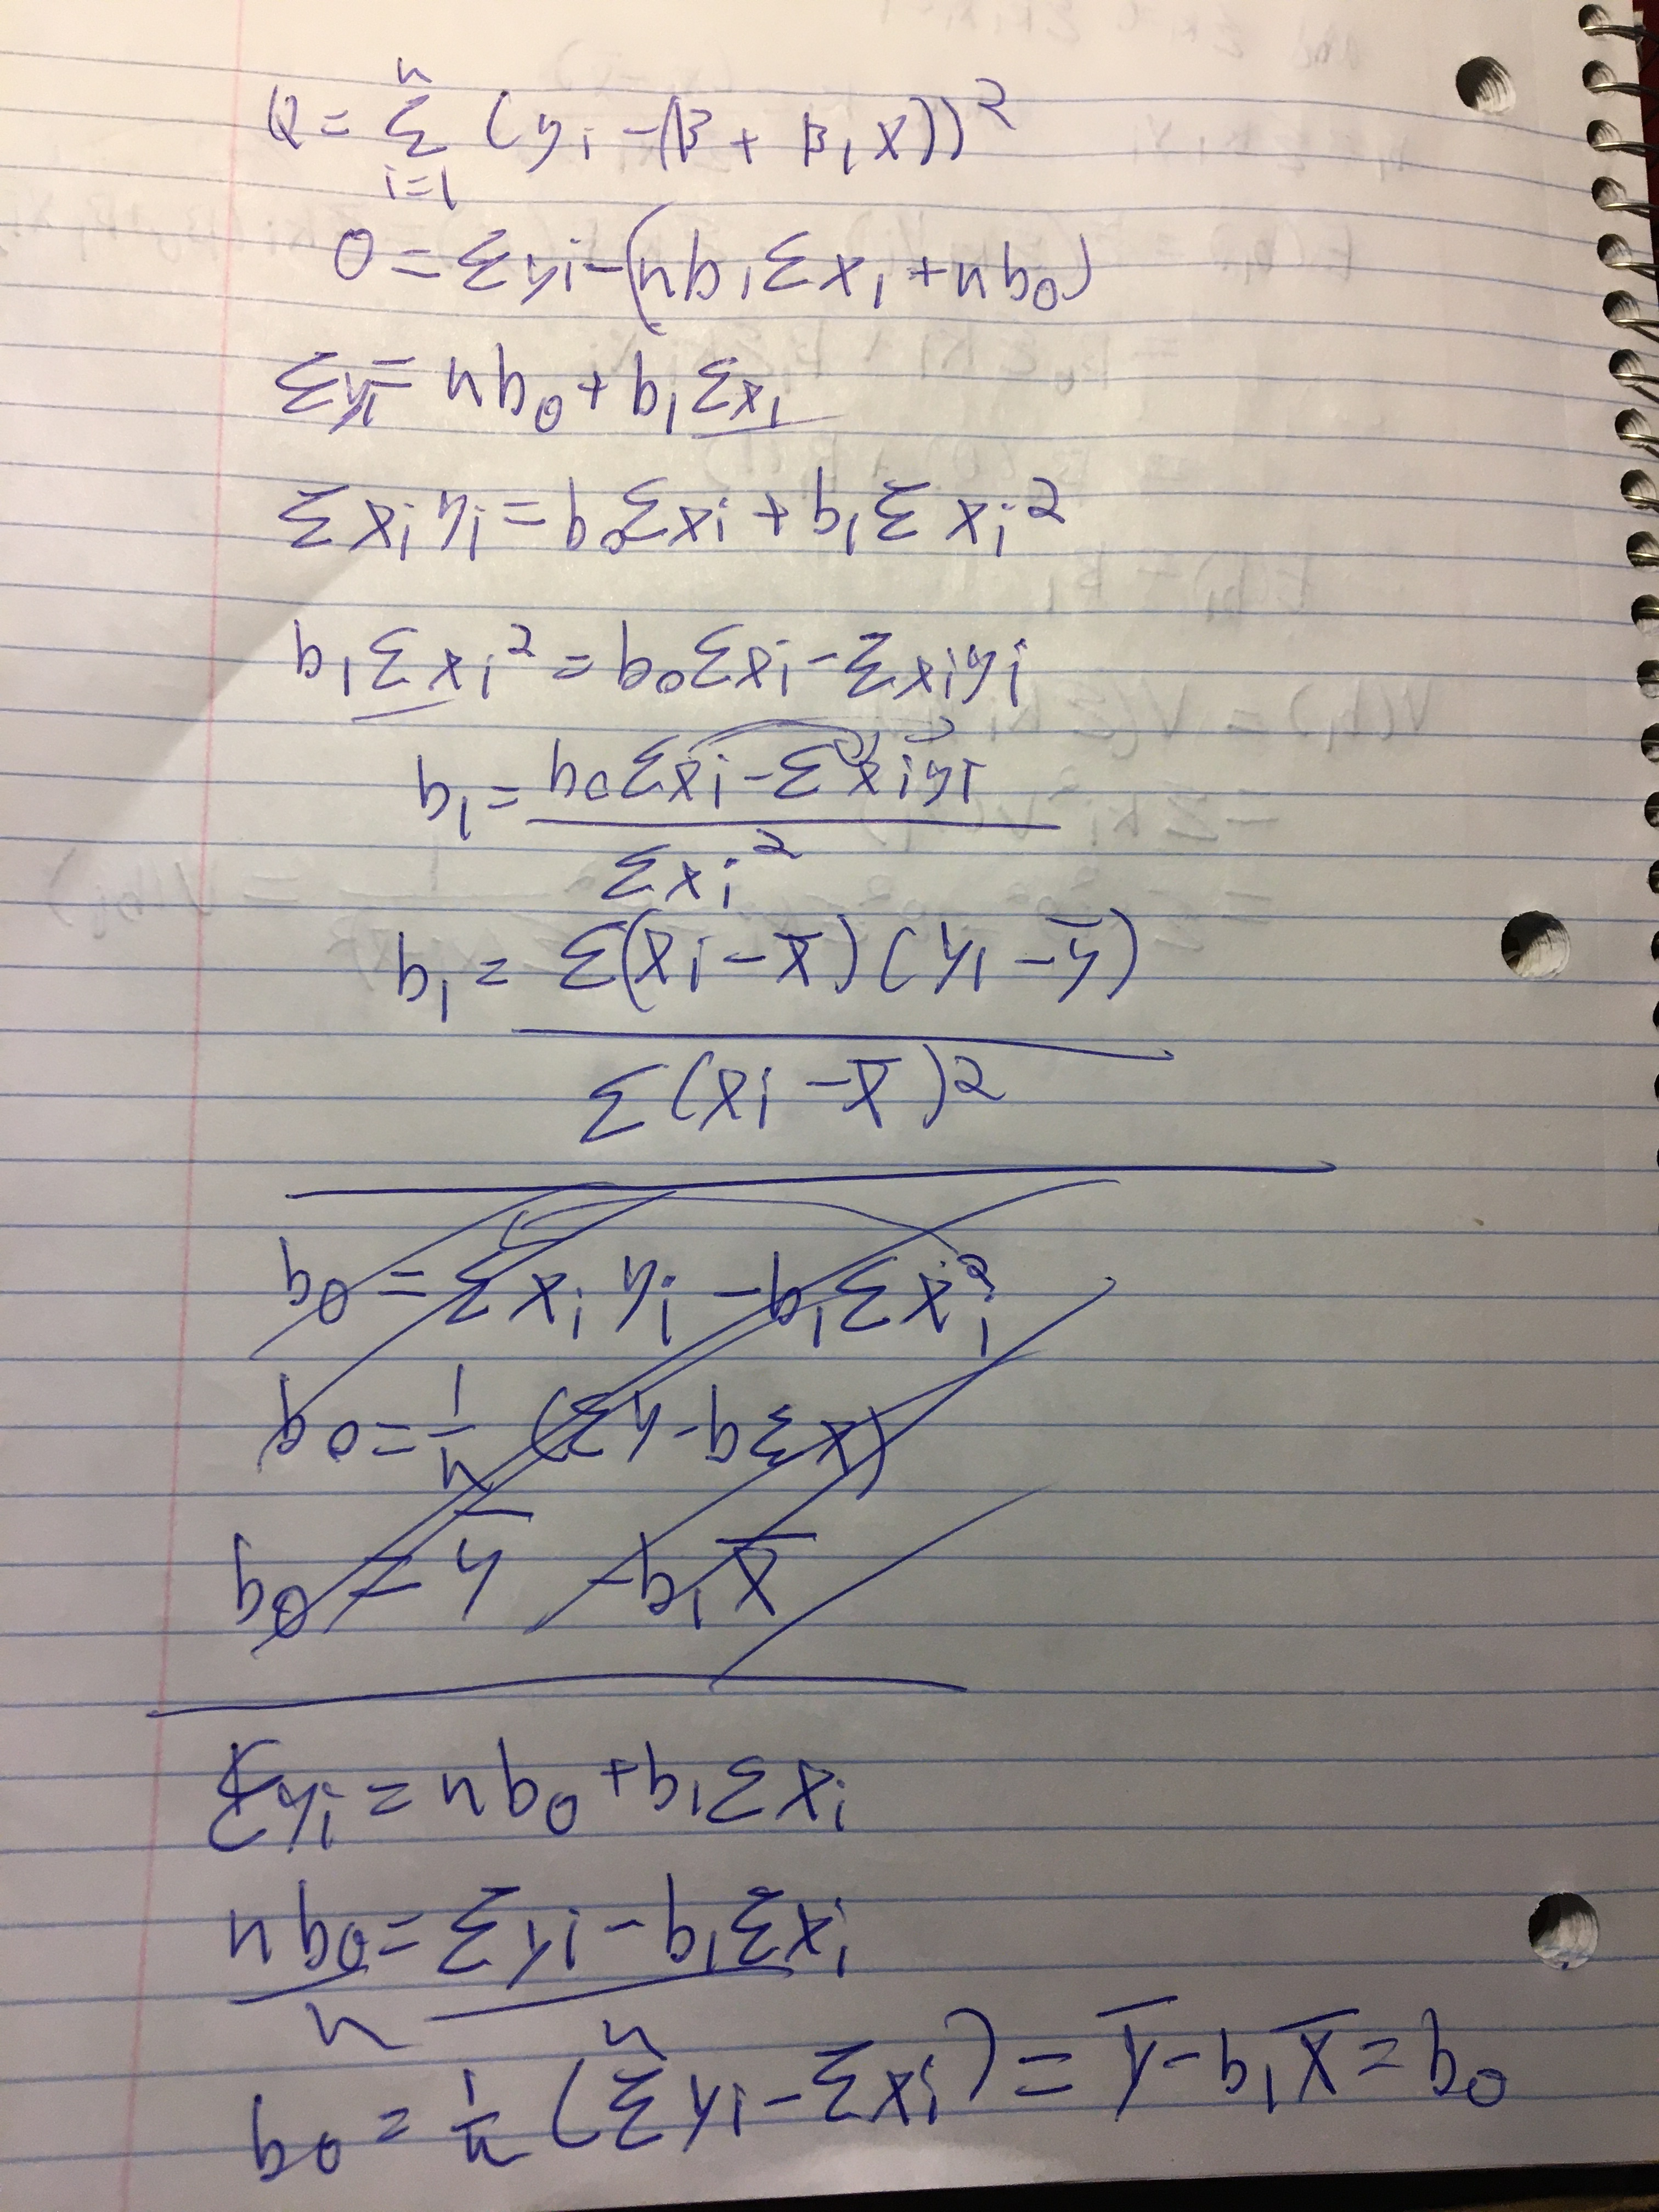
\includegraphics{/Users/philipsweet/Google Drive/2019-2020/Regression/HW1_1b.JPG}
\caption{Drawing.}
\end{figure}

\hypertarget{section-1}{%
\section{\texorpdfstring{\textbf{2}}{2}}\label{section-1}}

derive the Expectation and Variance of b1

\begin{figure}
\centering
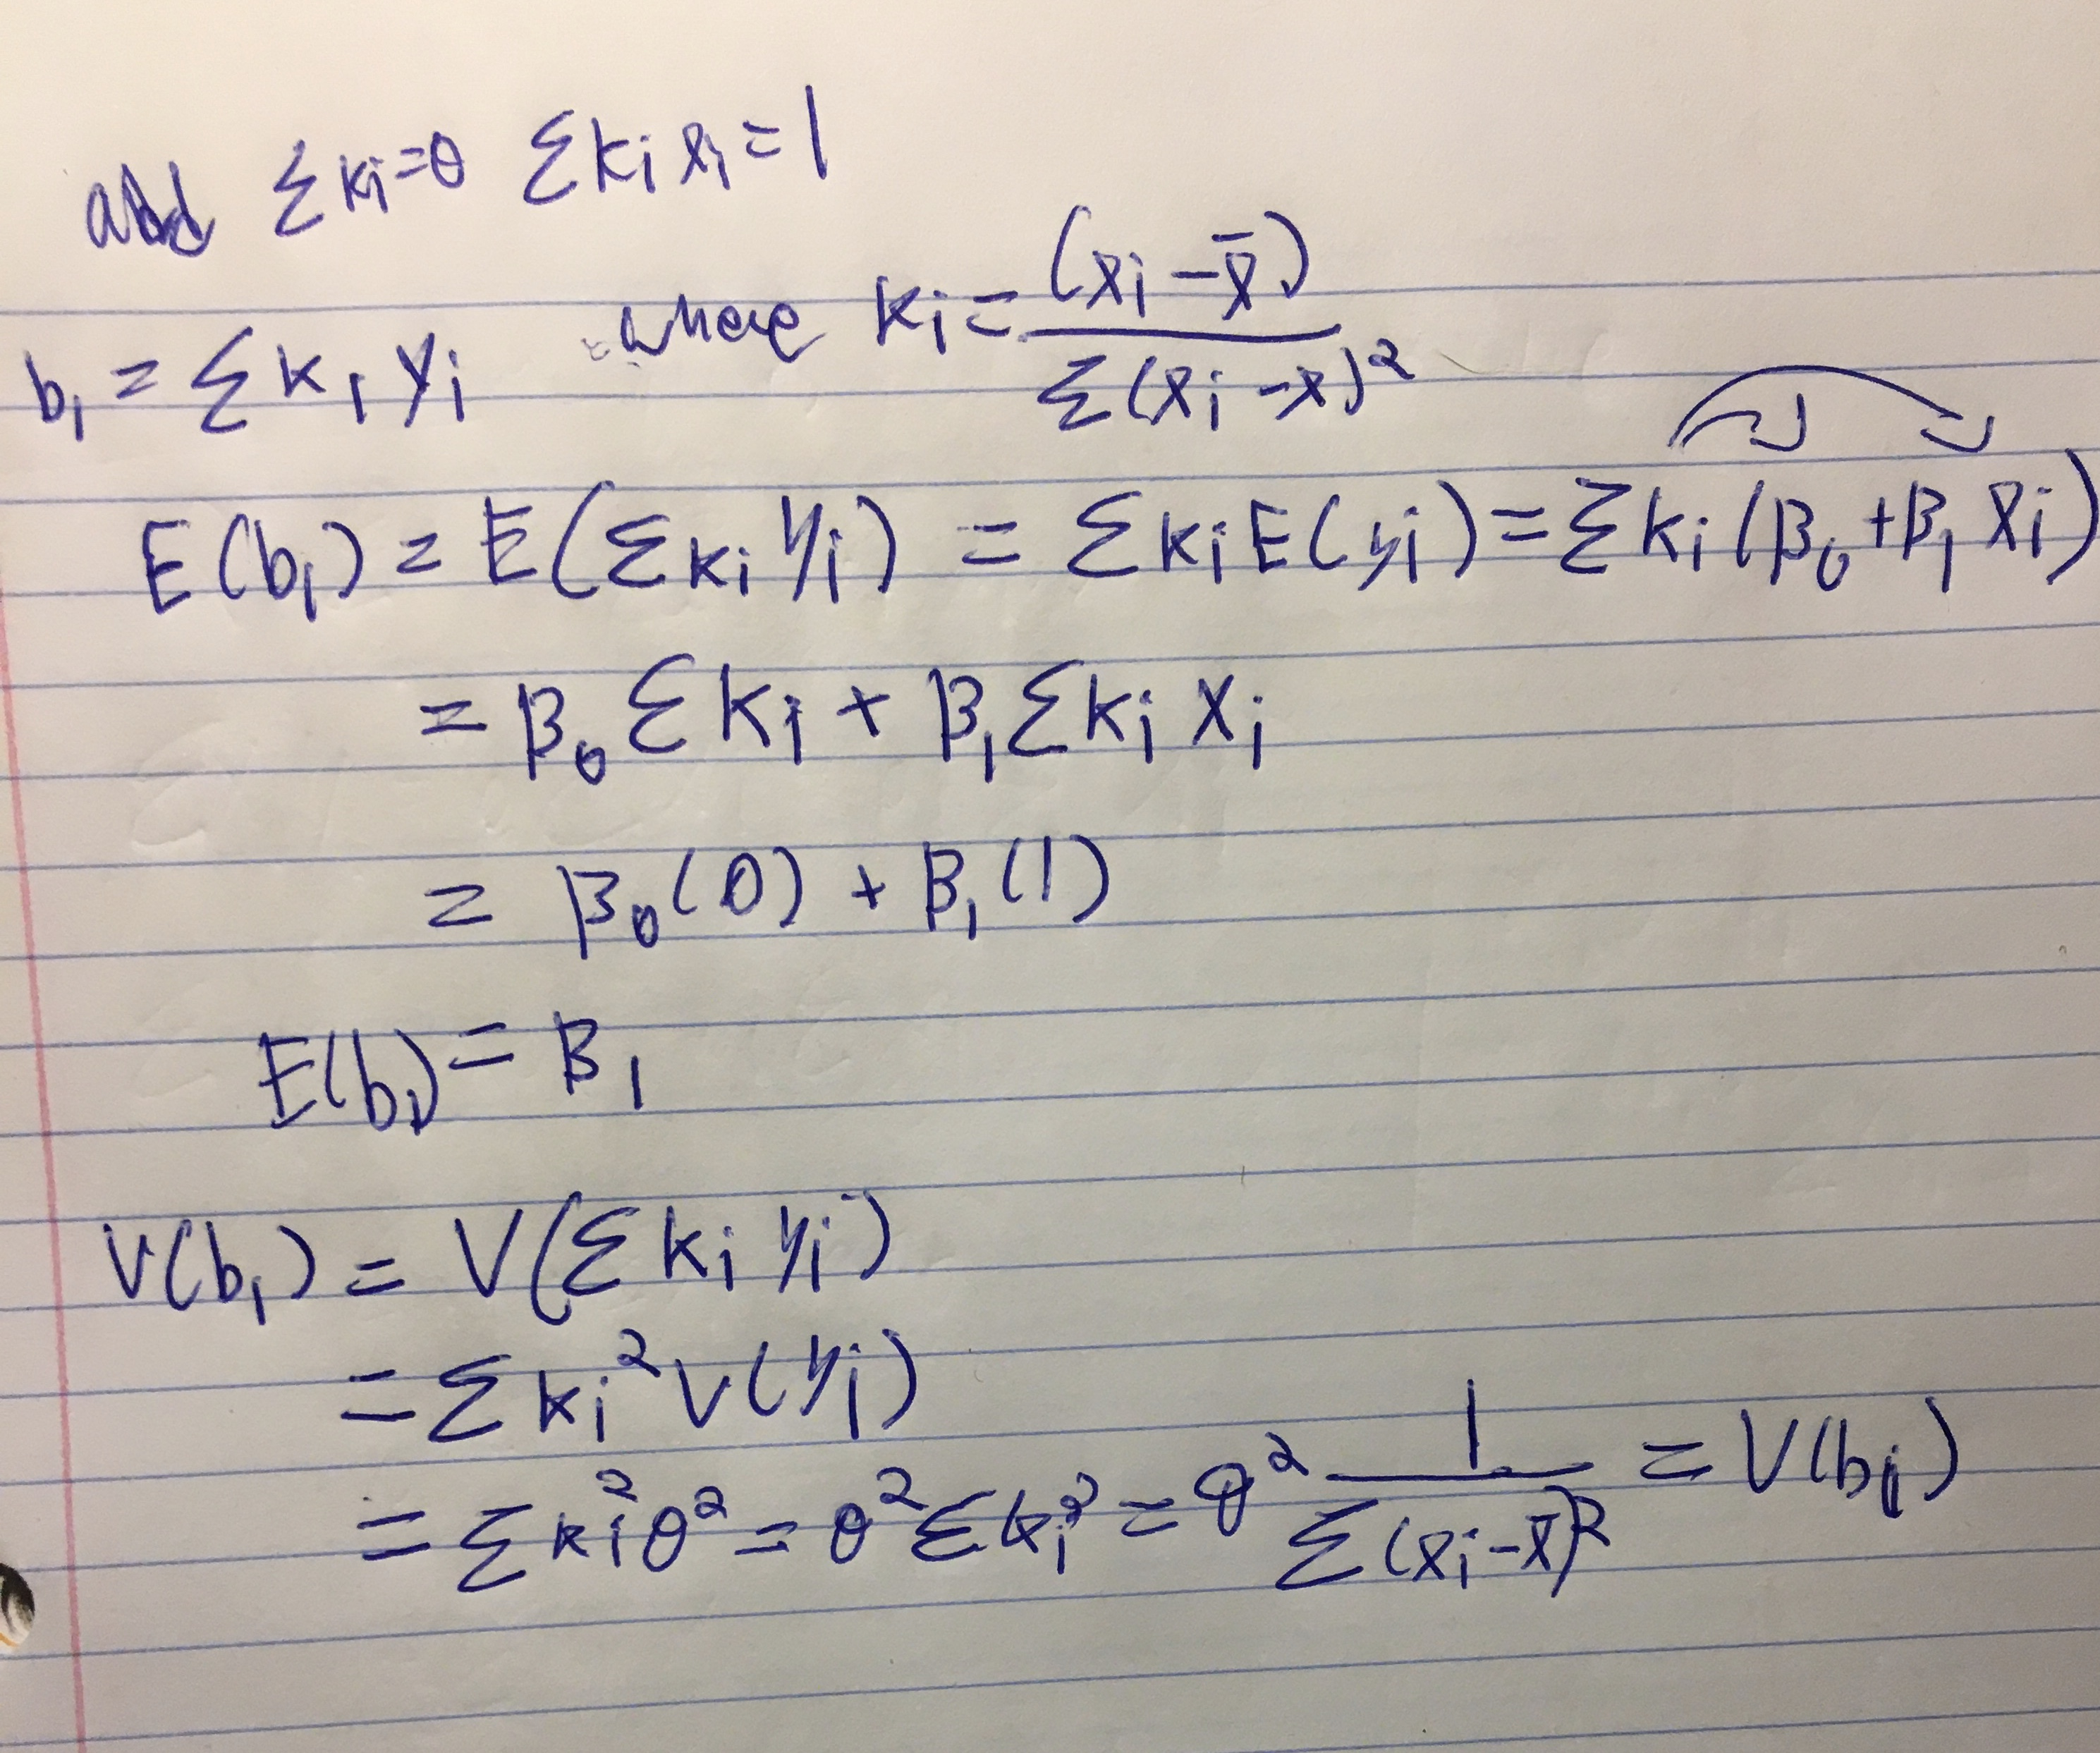
\includegraphics{/Users/philipsweet/Google Drive/2019-2020/Regression/HW1_2.JPG}
\caption{Drawing.}
\end{figure}

\hypertarget{section-2}{%
\section{\texorpdfstring{\textbf{3}}{3}}\label{section-2}}

Consider the normal error regression model\ldots{}
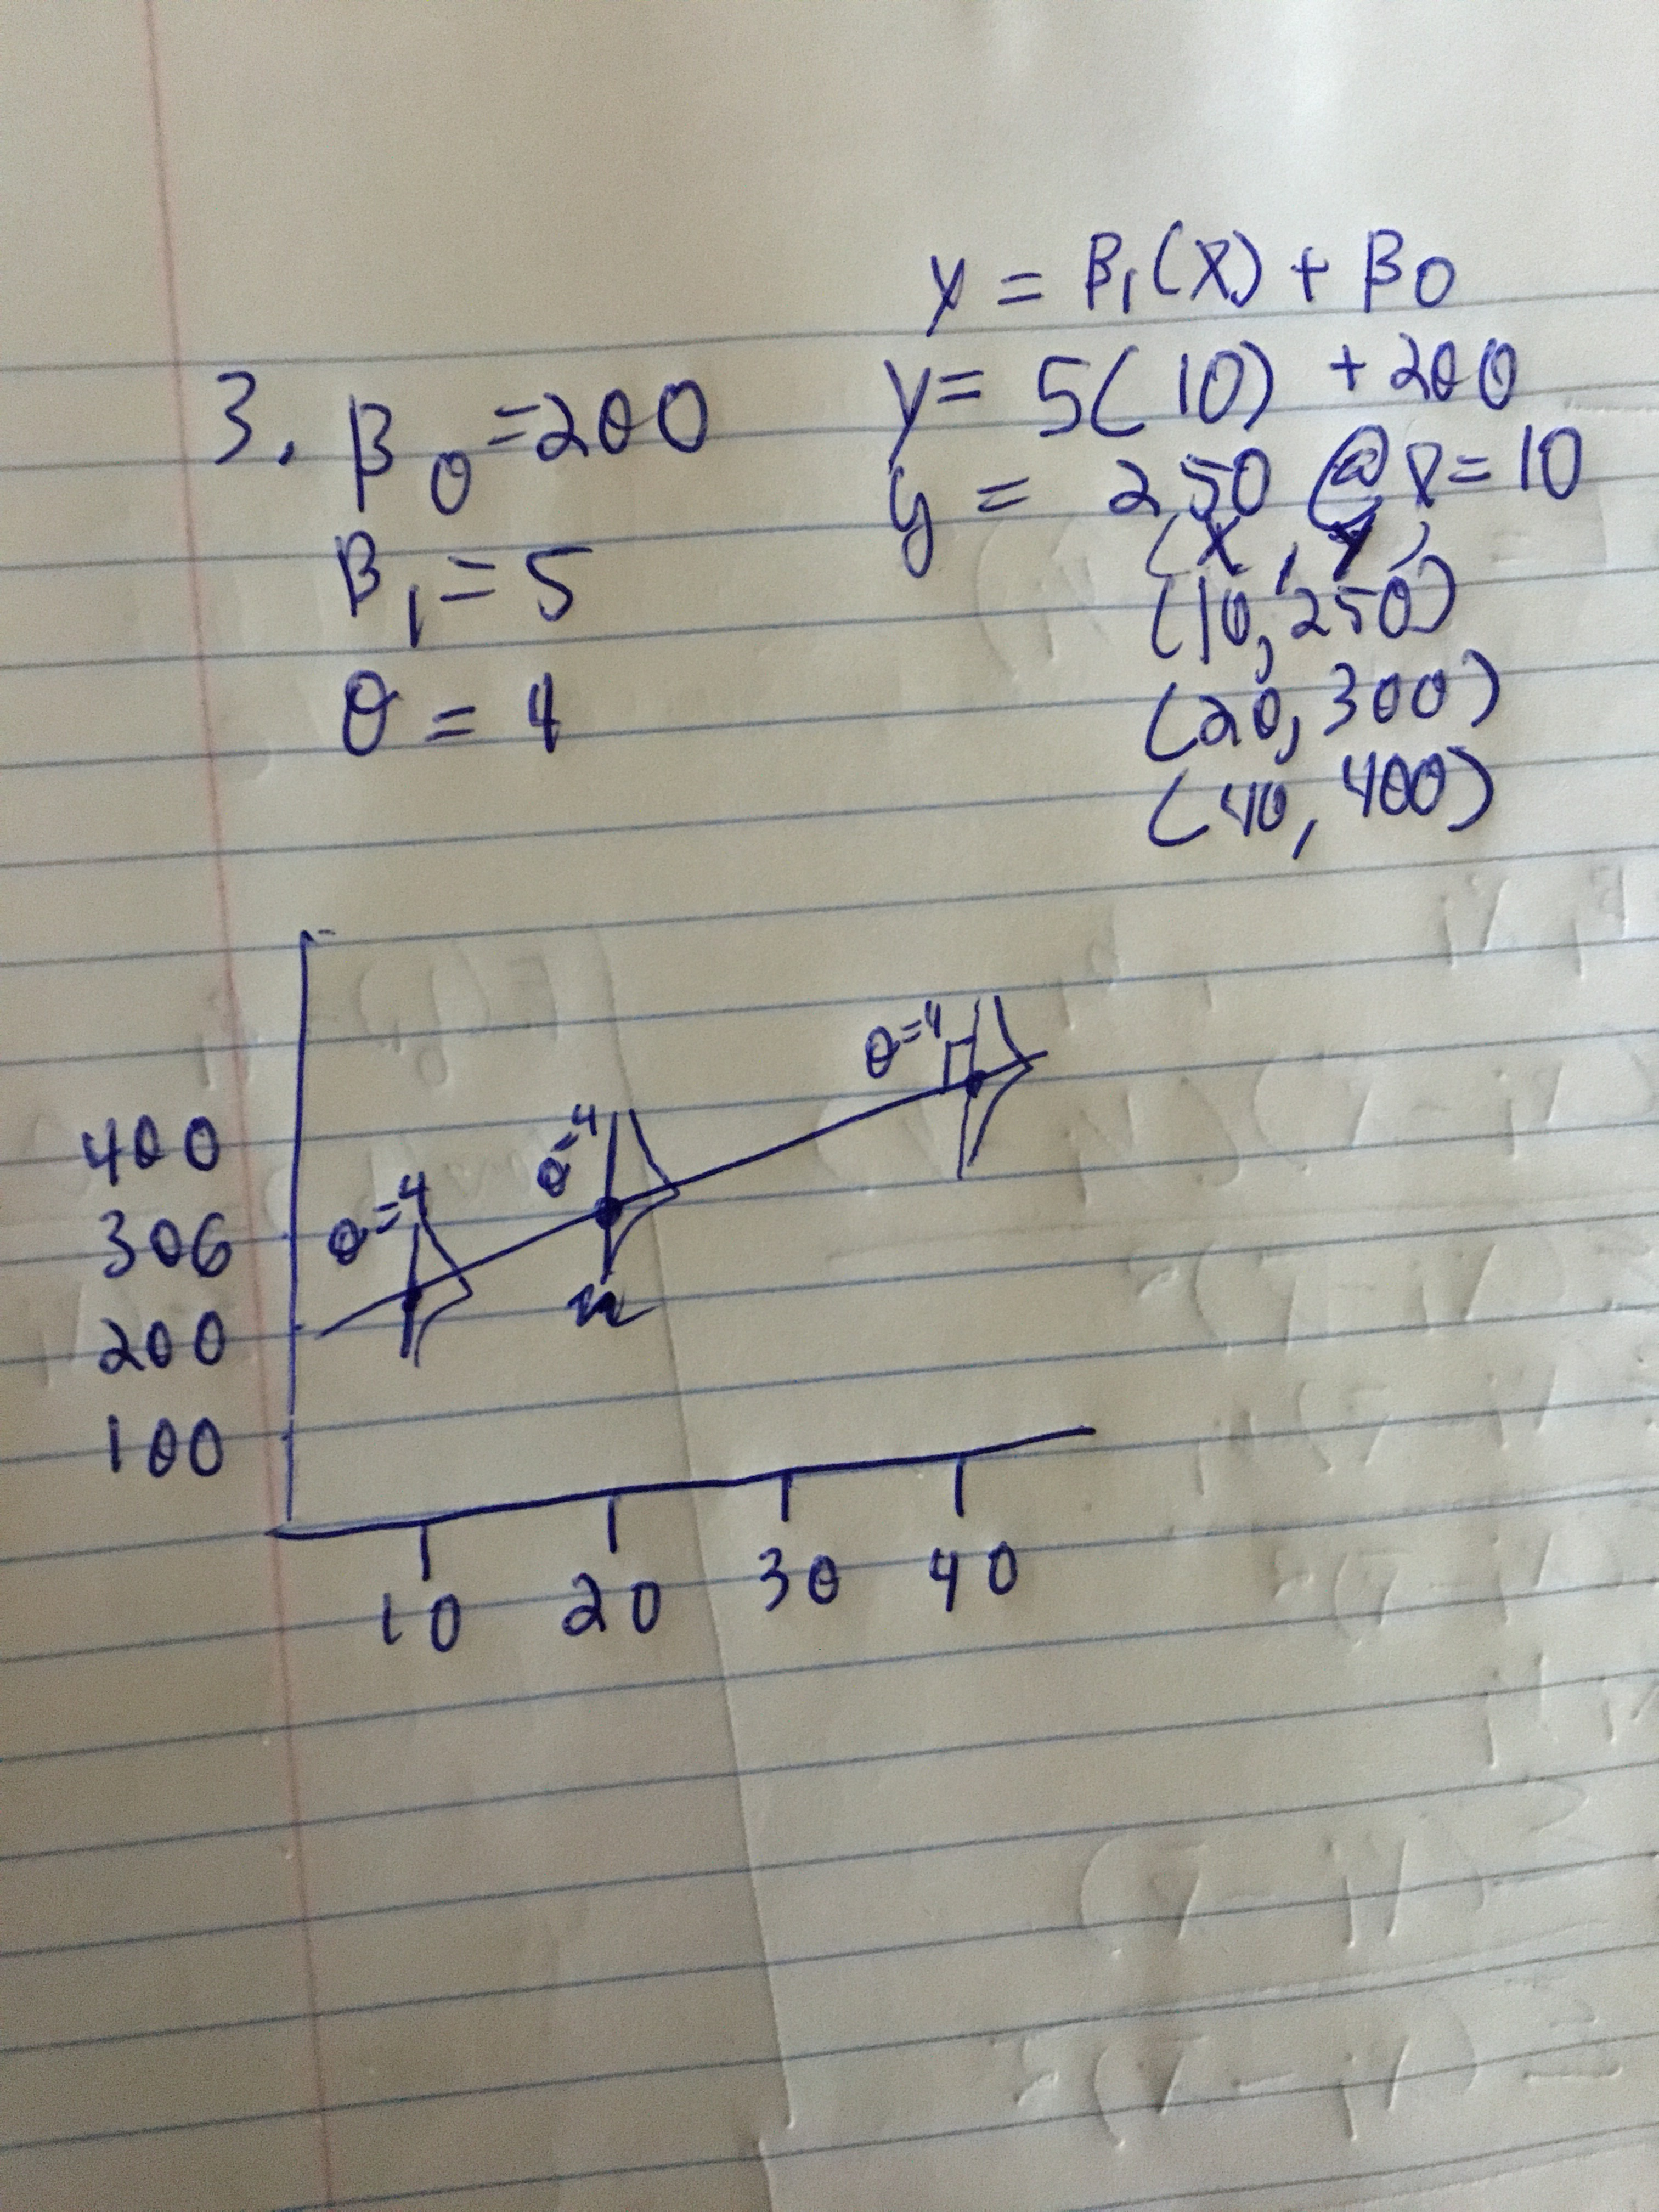
\includegraphics{/Users/philipsweet/Google Drive/2019-2020/Regression/HW1_3.JPG}

\hypertarget{section-3}{%
\section{\texorpdfstring{\textbf{4}}{4}}\label{section-3}}

\hypertarget{a}{%
\subsection{A}\label{a}}

In this situation, the B0 would be relatively meaningless because B0
represents how far away a person who was zero year old would be able to
read the a highway sign. No one who is zero years old is driving,
however, if they were, this model predicts that they would be able to
read it from 576 feet away.

\hypertarget{b}{%
\subsection{B}\label{b}}

In this situation, the B1 represents the negative change in distance (in
feet) per year of age from which a driver can read a highway sign. B1's
value of 3 means that for each unit increase in age, the distance a
driver can read a highway sign from decreases

\hypertarget{c}{%
\subsection{C}\label{c}}

\begin{figure}
\centering
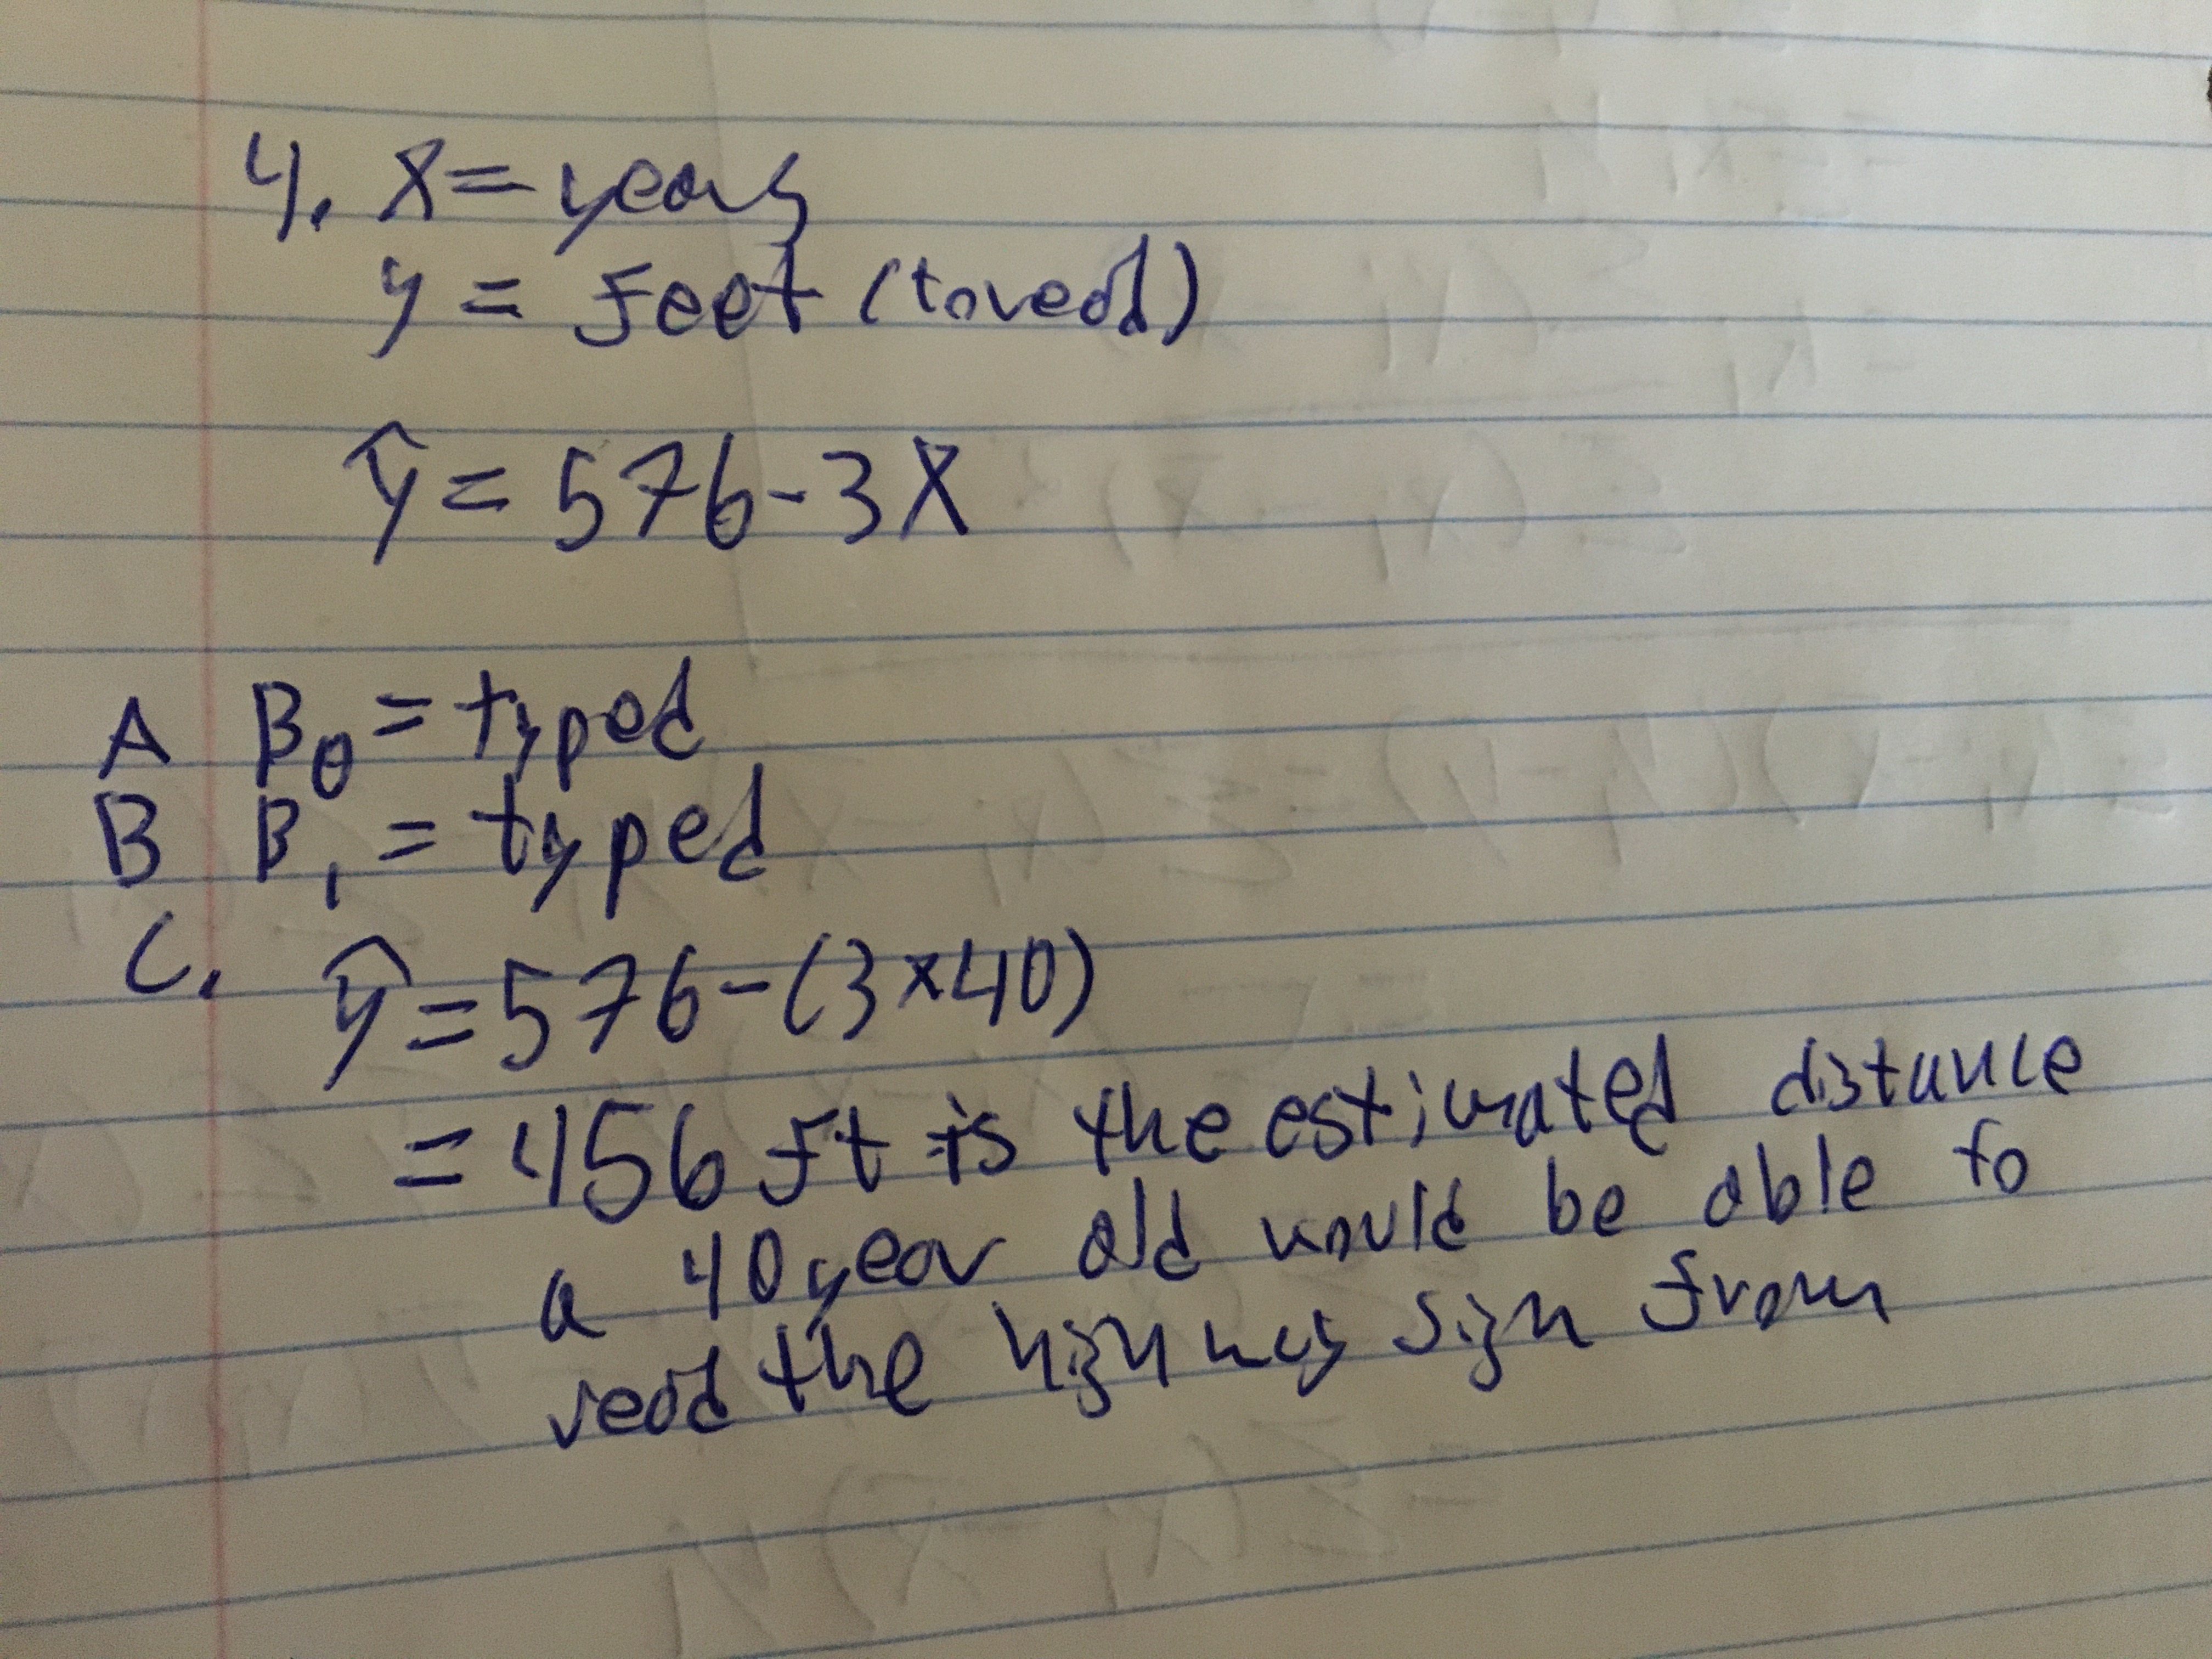
\includegraphics{/Users/philipsweet/Google Drive/2019-2020/Regression/HW1_4.JPG}
\caption{Drawing.}
\end{figure}

\hypertarget{d}{%
\subsection{D}\label{d}}

Residual = 44

\hypertarget{e}{%
\subsection{E}\label{e}}

D was an under-estimate

\hypertarget{section-4}{%
\section{\texorpdfstring{\textbf{5}}{5}}\label{section-4}}

Stop has data on the speed (X, in mph) and stopping distance (Y, in ft)
of 50 cars.

\begin{Shaded}
\begin{Highlighting}[]
\KeywordTok{read.csv}\NormalTok{(}\StringTok{"Stop.csv"}\NormalTok{, }\DataTypeTok{header =} \OtherTok{TRUE}\NormalTok{) ->}\StringTok{ }\NormalTok{data}
\end{Highlighting}
\end{Shaded}

\hypertarget{a.}{%
\subsection{A.}\label{a.}}

In this scatter plot, you can see that there is a positive linear
relationship between current speed and breaking distance.

\begin{Shaded}
\begin{Highlighting}[]
\KeywordTok{plot}\NormalTok{(data}\OperatorTok{$}\NormalTok{speed, }
\NormalTok{     data}\OperatorTok{$}\NormalTok{dist, }
     \DataTypeTok{main=}\StringTok{"Distance Requried to Break"}\NormalTok{,}
    \DataTypeTok{xlab=}\StringTok{"Speed (mph)"}\NormalTok{,}
    \DataTypeTok{ylab=}\StringTok{"Stopping Distance (ft)"}\NormalTok{)}
\end{Highlighting}
\end{Shaded}

\includegraphics{HW1_files/figure-latex/unnamed-chunk-2-1.pdf}

\hypertarget{b.}{%
\subsection{B.}\label{b.}}

Here we will calculate the sum of squares

\begin{Shaded}
\begin{Highlighting}[]
\NormalTok{n <-}\KeywordTok{length}\NormalTok{(data) }
\NormalTok{X <-data}\OperatorTok{$}\NormalTok{speed}
\NormalTok{Y <-data}\OperatorTok{$}\NormalTok{dist}

\CommentTok{## find the means of both vars}
\NormalTok{mean_x <-}\KeywordTok{mean}\NormalTok{(X)}
\NormalTok{mean_y <-}\KeywordTok{mean}\NormalTok{(Y)}

\CommentTok{## find the variance of each var}
\NormalTok{var_x <-}\KeywordTok{var}\NormalTok{(X)}
\NormalTok{var_y <-}\KeywordTok{var}\NormalTok{(Y)}

\NormalTok{cov_xy <-}\KeywordTok{cov}\NormalTok{(X,Y) }

\CommentTok{# finbd the sum of squares}
\NormalTok{SS_xx <-(n}\DecValTok{-1}\NormalTok{)}\OperatorTok{*}\NormalTok{var_x }
\NormalTok{SS_xy <-(n}\DecValTok{-1}\NormalTok{)}\OperatorTok{*}\NormalTok{cov_xy }
\NormalTok{SS_yy <-(n}\DecValTok{-1}\NormalTok{)}\OperatorTok{*}\NormalTok{var_y  }

\CommentTok{## solve for estimaters }
\NormalTok{b1 <-SS_xy}\OperatorTok{/}\NormalTok{SS_xx }
\NormalTok{b0 <-mean_y }\OperatorTok{-}\NormalTok{b1}\OperatorTok{*}\NormalTok{mean_x }
\NormalTok{yhat <-b0 }\OperatorTok{+}\StringTok{ }\NormalTok{b1}\OperatorTok{*}\NormalTok{X }
\NormalTok{e <-Y}\OperatorTok{-}\NormalTok{yhat  }
\NormalTok{SSE <-}\KeywordTok{sum}\NormalTok{(e}\OperatorTok{^}\DecValTok{2}\NormalTok{) }
\NormalTok{MSE <-SSE}\OperatorTok{/}\NormalTok{(n}\DecValTok{-2}\NormalTok{) }
\NormalTok{s <-}\KeywordTok{sqrt}\NormalTok{(MSE)  }
\end{Highlighting}
\end{Shaded}

The slope (b1) = 3.9324088 and the intercept (b0) = -17.5790949

Thus the est. regression equation is y = 3.9324088x -17.5790949

\hypertarget{c.}{%
\subsection{C.}\label{c.}}

\begin{Shaded}
\begin{Highlighting}[]
\KeywordTok{plot}\NormalTok{(X,Y,}
    \DataTypeTok{xlim=}\KeywordTok{c}\NormalTok{(}\DecValTok{0}\NormalTok{,}\DecValTok{25}\NormalTok{), }
    \DataTypeTok{main=}\StringTok{"Distance Requried to Break"}\NormalTok{,}
    \DataTypeTok{xlab=}\StringTok{"Speed (mph)"}\NormalTok{,}
    \DataTypeTok{ylab=}\StringTok{"Stopping Distance (ft)"}\NormalTok{) }
\KeywordTok{abline}\NormalTok{(}\DataTypeTok{a=}\NormalTok{b0,}\DataTypeTok{b=}\NormalTok{b1)  }
\end{Highlighting}
\end{Shaded}

\includegraphics{HW1_files/figure-latex/unnamed-chunk-4-1.pdf}

When we lay the regression line overe the data, we can see that line
seems to estiamte the stopping distance well at ll speeds provided in
the data.

\hypertarget{d-1}{%
\subsection{D}\label{d-1}}

When using the linear model function in R (lm) we can see that \ldots{}

\begin{Shaded}
\begin{Highlighting}[]
\NormalTok{lm_a <-}\StringTok{ }\KeywordTok{lm}\NormalTok{(Y }\OperatorTok{~}\StringTok{ }\NormalTok{X)}

\KeywordTok{summary}\NormalTok{(lm_a)}
\end{Highlighting}
\end{Shaded}

\begin{verbatim}
## 
## Call:
## lm(formula = Y ~ X)
## 
## Residuals:
##     Min      1Q  Median      3Q     Max 
## -29.069  -9.525  -2.272   9.215  43.201 
## 
## Coefficients:
##             Estimate Std. Error t value Pr(>|t|)    
## (Intercept) -17.5791     6.7584  -2.601   0.0123 *  
## X             3.9324     0.4155   9.464 1.49e-12 ***
## ---
## Signif. codes:  0 '***' 0.001 '**' 0.01 '*' 0.05 '.' 0.1 ' ' 1
## 
## Residual standard error: 15.38 on 48 degrees of freedom
## Multiple R-squared:  0.6511, Adjusted R-squared:  0.6438 
## F-statistic: 89.57 on 1 and 48 DF,  p-value: 1.49e-12
\end{verbatim}

\ldots{} which (in the Coefficients column) generates the same estimates
for B1 and B0 is what we had manually calculated above.

\hypertarget{e-1}{%
\subsection{E}\label{e-1}}

In this context the slope (b1) represents an increased spotting distance
of 3.9 feet for every extra mile per hout in speed. The intercept (b0)
in this case is of no meaning, as a car that was not moving (speed = 0)
would require no distance to stop, but it does suggest that the model
may be less informative at lower speeds.

\hypertarget{f}{%
\subsection{F}\label{f}}

\begin{Shaded}
\begin{Highlighting}[]
\NormalTok{conf <-}\StringTok{ }\KeywordTok{confint}\NormalTok{(lm_a, }\StringTok{'X'}\NormalTok{, }\DataTypeTok{level=}\FloatTok{0.95}\NormalTok{)}
\end{Highlighting}
\end{Shaded}

The 95\% confidence interval for the slope is ( 3.0969643, 4.7678532 )

To a conduct a hypothesis test for a significant linear relationship
between starting speed and stopping distance, we can use\ldots{}

Ho: b1 = 0

Ha: b1 ≠ 0

Using the 95\% coffidence interval generated above ( 3.0969643,
4.7678532 ) we can see that 0 doesn't reside within this interval, thus
we can reject the null hypthesis (Ha) that b1 = 0 and state that there
is a postive linear relationship between speed and stopping distance.


\end{document}
